\chapter{Sistemas de Unidades de Medidas}
O Sistema Métrico é um sistema internacional de medições que determina as unidades a serem utilizadas por cada uma das medidas, além de suas transformações, Nesse capitulo voçê verá que cada medida tem sua unidade padrão, de acordo com o Sistema Internacional de Unidades.

\section{Medidas de Comprimento}
As medidas de comprimento são os mecanismos de medição mais utilizados. A unidade fundamental das medidas de comprimento é o metro ($\mathrm{m}$). 
\begin{multicols}{2}
	\subsection{Múltiplos de Metro}
		\begin{itemize}
			\item Quilômetro ($\mathrm{km}$) $= 1000 \mathrm{m} = 10^3 \mathrm{m}$
			\item Hectômetro ($\mathrm{hm}$) $= 100 \mathrm{m} = 10^2\mathrm{m}$
			\item Decâmetro ($\mathrm{dam}$) $= 10 \mathrm{m}$ 
			
		\end{itemize}

	\subsection{Submúltiplos de Metro}
		\begin{itemize}
			\item Dec\'imetro ($\mathrm{dm}$) $= 0,1\mathrm{m} = 10^{-1}\mathrm{m}$
			\item Centímetro ($\mathrm{cm}$) $= 0,01\mathrm{m} = 10^{-2}\mathrm{m}$
			\item Milímetro ($\mathrm{mm}$) $= 0,001\mathrm{m} = 10^{-3}\mathrm{m}$
		\end{itemize}
\columnbreak
     \bigskip
     \noindent   % Very important in case that \parindent is not 0pt
     \begin{minipage}{\linewidth}
            \centering 
            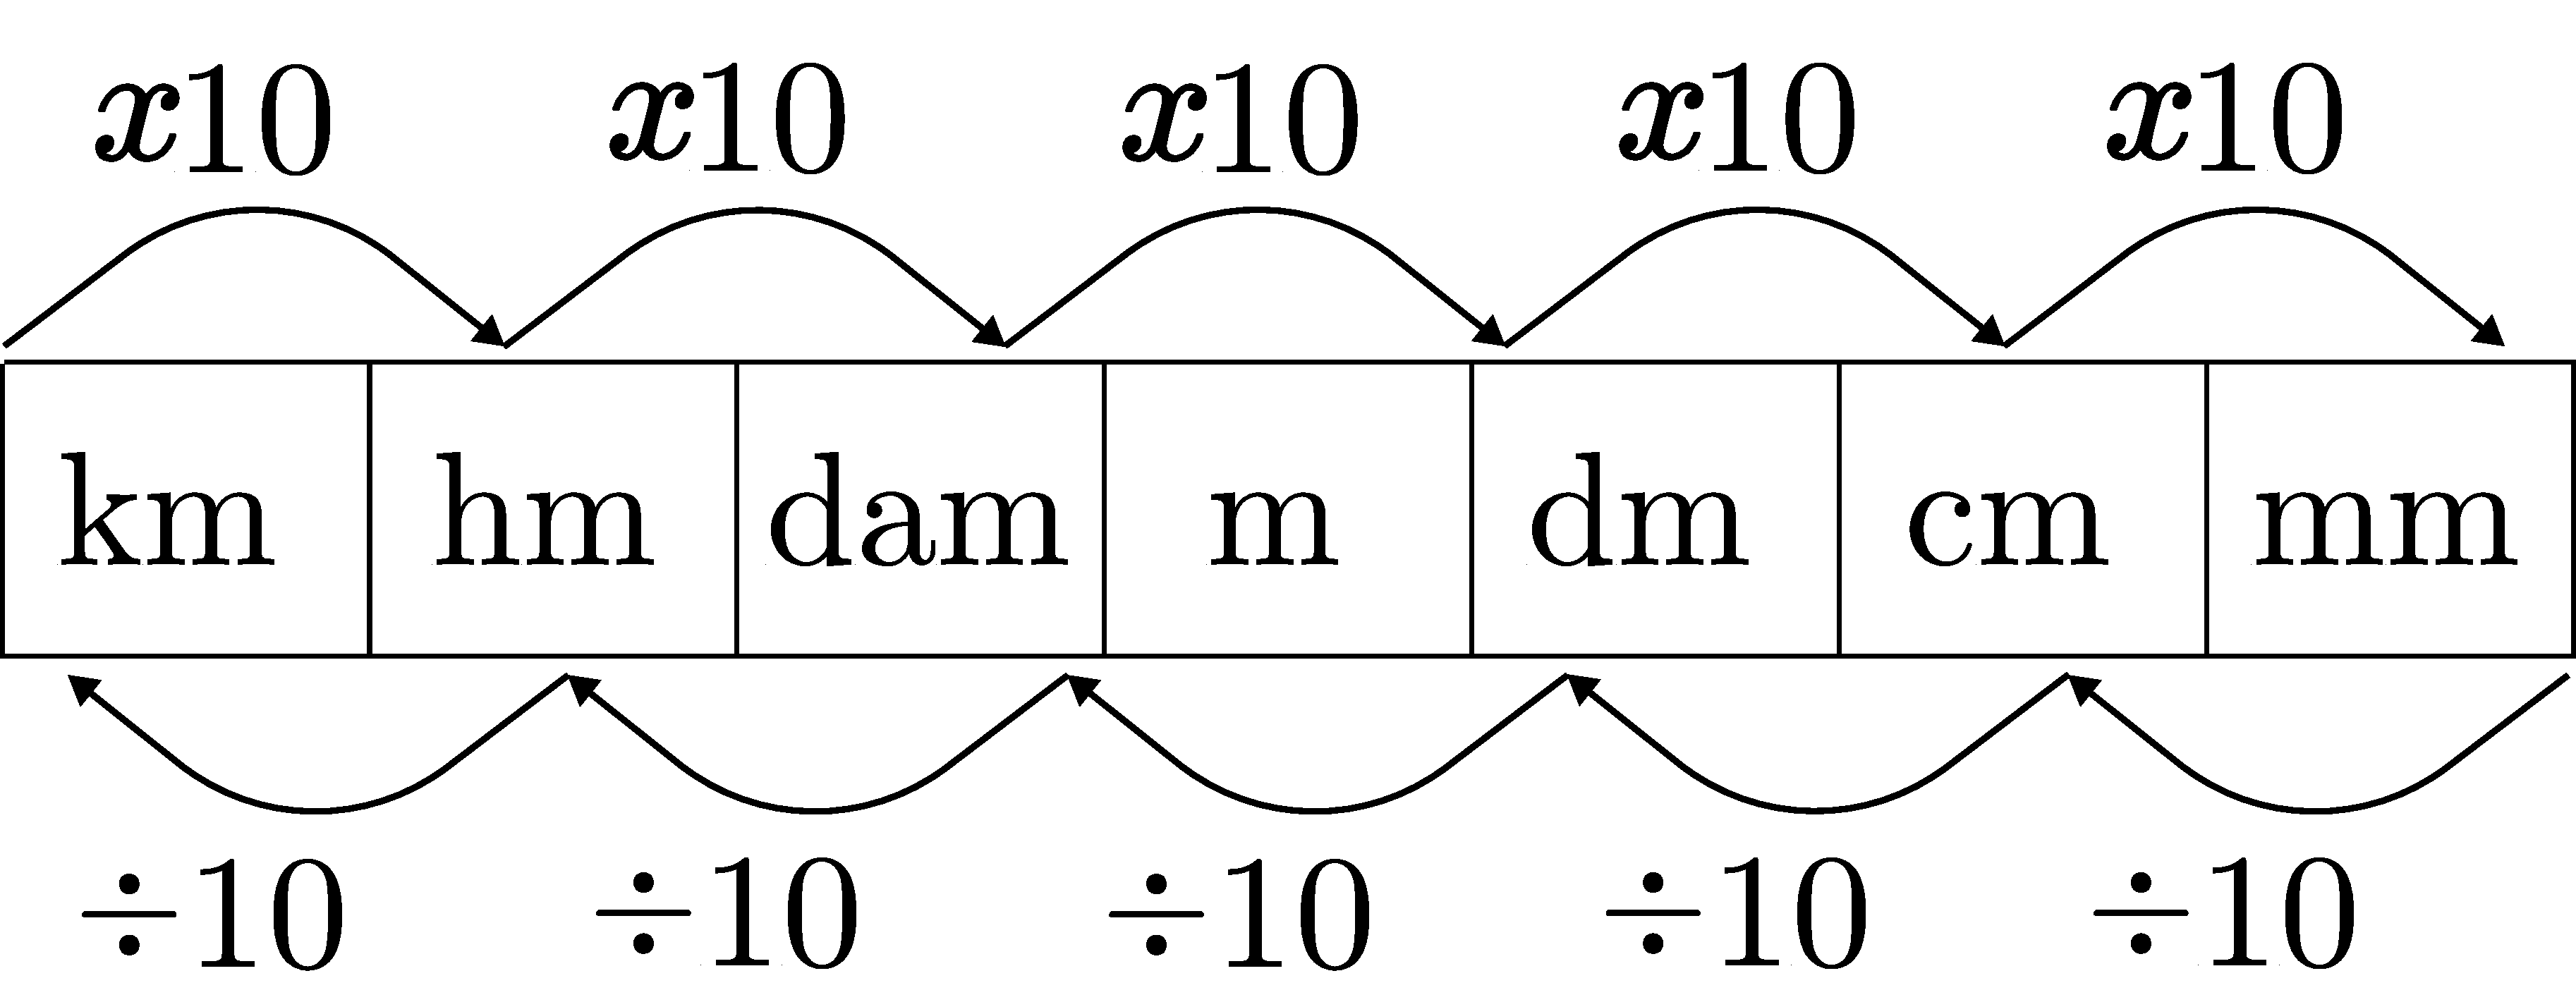
\includegraphics[width=0.8\textwidth]{imagens/matematicaBasica/sistemaDeUnidades/MultiplosDeMetro.pdf}
     \end{minipage}
   \end{multicols}


\section{Medidas de Superfície}
As medidas de superfície são as utilizadas na medição de
áreas. Sua unidade fundamental é o metro quadrado ($\mathrm{m}^2$).
    \subsection{Múltiplos de Metro Quadrado ($\mathrm{m}^2$)}
		\begin{itemize}
			\item Quilômetro quadrado ($\mathrm{km}^2$) $= 1.000.000 \mathrm{m}^2 = 10^6 \mathrm{m}^2$
			\item Hectômetro quadrado ($\mathrm{hm}^2$) $= 10.000 \mathrm{m}^2 = 10^4 \mathrm{m}^2$
			\item Decâmetro quadrado ($\mathrm{dam}^2$) $= 100 \mathrm{m}^2 = 10^2 \mathrm{m}^2$
		\end{itemize}
		
\newpage
	\subsection{Submúltiplos de Metro Quadrado}
		\begin{itemize}
			\item Decímetro quadrado ($\mathrm{dm}^2$) $= 0,01\mathrm{m}^2 = 10^{-2}\mathrm{m}^2$
			\item centímetro quadrado ($\mathrm{cm}^2$) $= 0,0001\mathrm{m}^2 = 10^{-4}\mathrm{m}^2$
			\item Milímetro quadrado ($\mathrm{mm}^2$) $= 0,000001\mathrm{m}^2 = 10^{-6}\mathrm{m}^2$
		\end{itemize}

    \begin{figure}[!h]
		    \centering 
            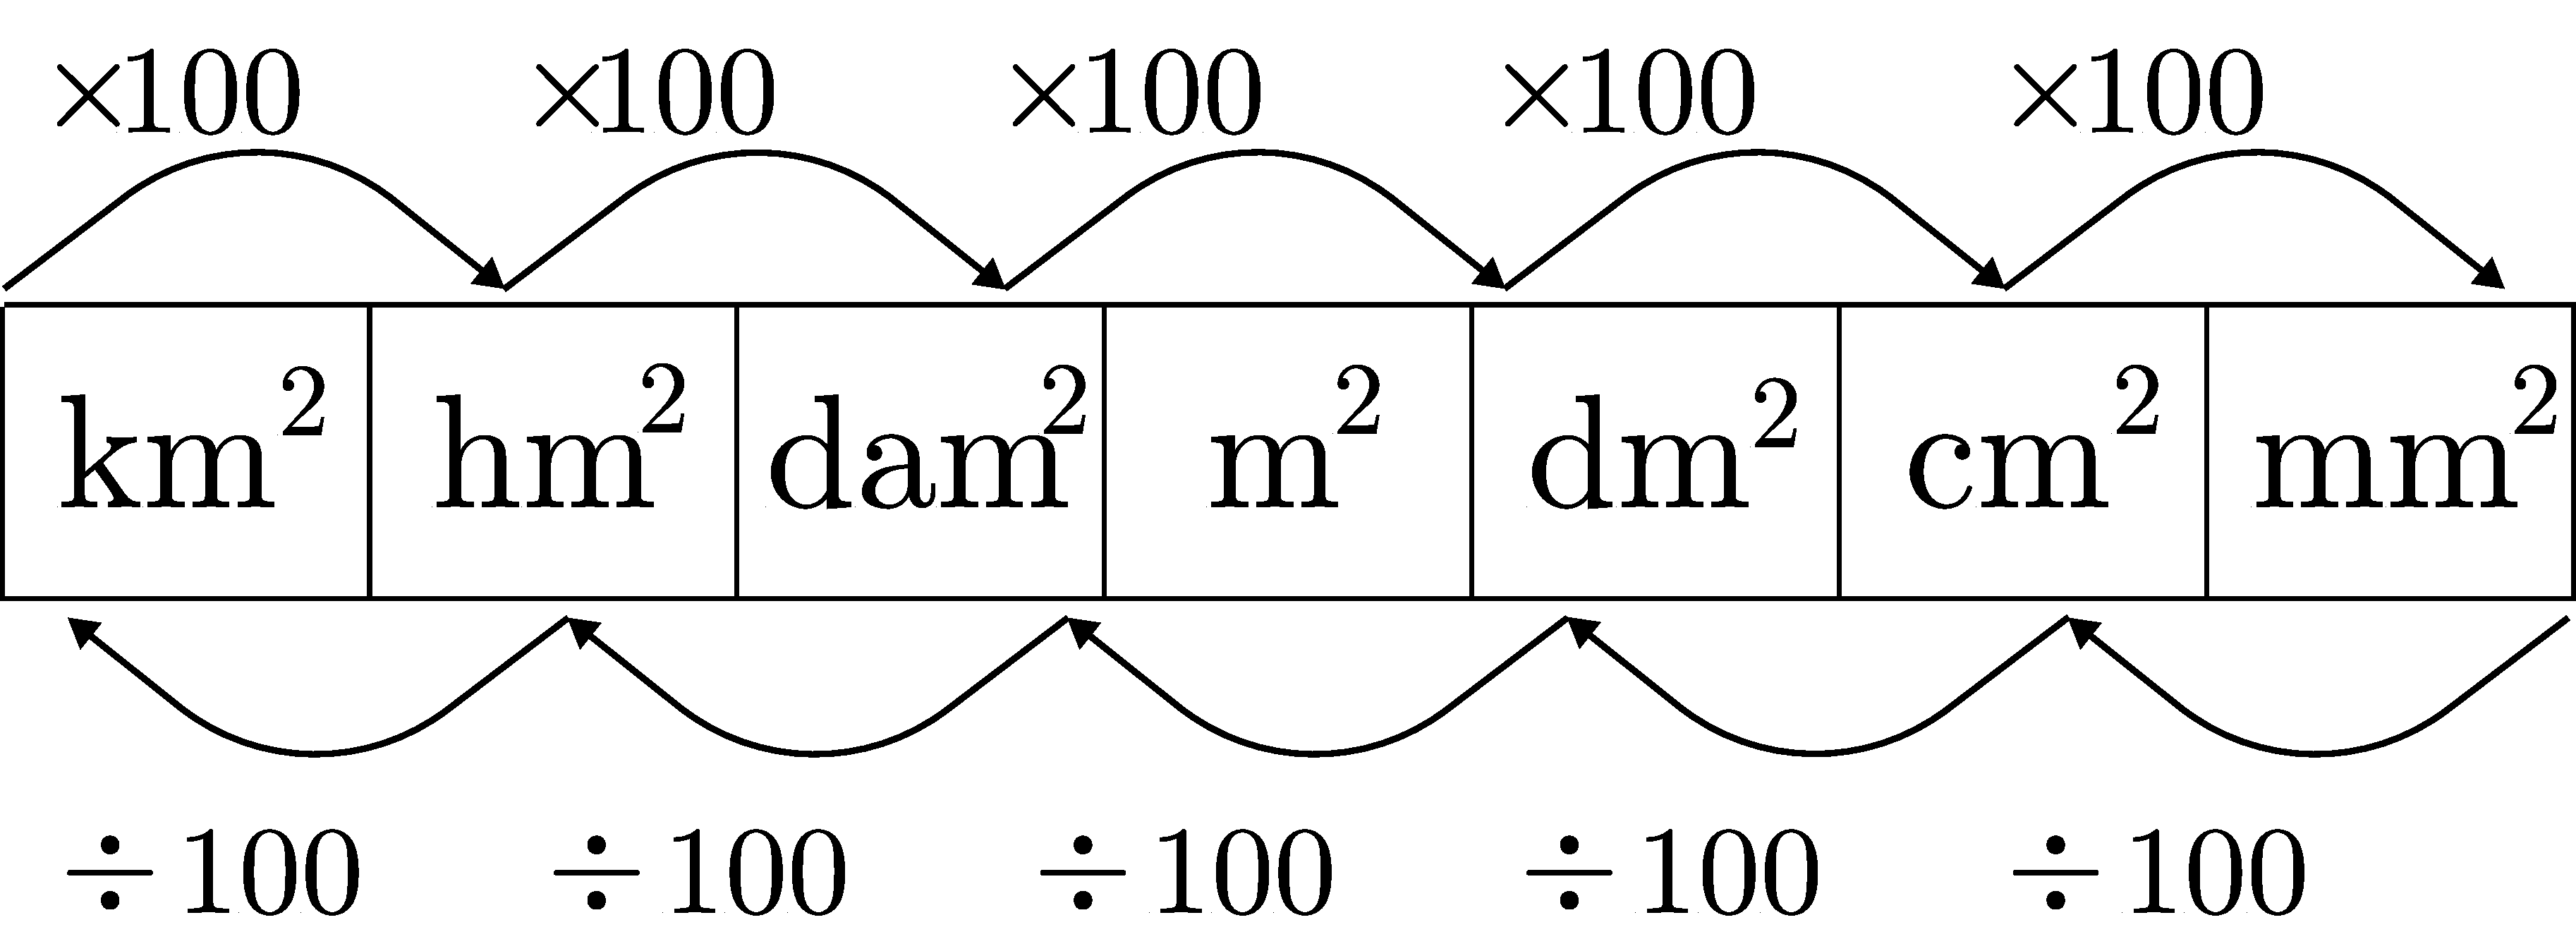
\includegraphics[width=0.4\textwidth]{imagens/matematicaBasica/sistemaDeUnidades/MultiplosDeMetroQuadrado.pdf}
		\end{figure}
		
\section{Medidas Agrárias}
Dentre as medidas de superfícies, existem as medidas
agrárias, que são mais utilizadas para medir áreas rurais. Sua
unidade fundamental é o are ($\mathrm{a}$).
	\begin{itemize}
		\item Centiare ($\mathrm{ca}$) $= 1\mathrm{m}^{2}=10^{0}\mathrm{m}^{2}$
		\item Are ($\mathrm{a}$) $= 100\mathrm{m}^{2} = 10^{2}\mathrm{m}^{2}$
		\item Hectare ($\mathrm{ha}$) $= 10000\mathrm{m}^{2} = 10^{4}\mathrm{m}^{2}$
	\end{itemize}

\section{Medidas de Volume} 
As medidas de volume são utilizadas para medir o espaço ocupado por um corpo tridimensional ou a sua capacidade de armazenar alguma substância. Você pode observar que essa medição é bastante usual em outras disciplinas, como por exemplo em química, as medidas de volume geralmente aparecem quando medimos quantidades de líquidos ou outras substancias. A unidade métrica tradicional de volume usada nesse caso é o litro ($\mathrm{l}$). Em termos
do SI, um litro é definido exatamente como $14$ decímetro cúbico.
\subsection{Múltiplos do Metro Cubico:}
		\begin{itemize}
		    \item Quilômetro cúbico ($\mathrm{km}^3$) $= 1.000.000.000 \mathrm{m}^3 = 10^9 \mathrm{m}^3$
		    \item Hectômetro cúbico ($\mathrm{hm}^3$) $= 1.000.000 \mathrm{m}^3 = 10^6 \mathrm{m}^3$
		    \item Decâmetro cúbico $(\mathrm{dam}^3) = 1.000 \mathrm{m}^3 = 10^3 \mathrm{m}^3$
		\end{itemize}
	
\subsection{Submúltiplos de Metros Cúbicos ($\mathrm{m}^3$)}
		\begin{itemize}
		    \item Decímetro cúbico $(\mathrm{dm}^3) = 0,001 \mathrm{m}^3 = 10^{-3} \mathrm{m}^3$
		    \item Centímetro cúbico $(\mathrm{cm}^3) = 0,000001 \mathrm{m}^3 = 10^{-6} \mathrm{m}^3$
		    \item Milímetro cúbico $(\mathrm{mm}^3) = 0,000000001 \mathrm{m}^3 = 10^{-9} \mathrm{m}^3$
		\end{itemize}
		
		\begin{figure}[!h]
		    \centering 
            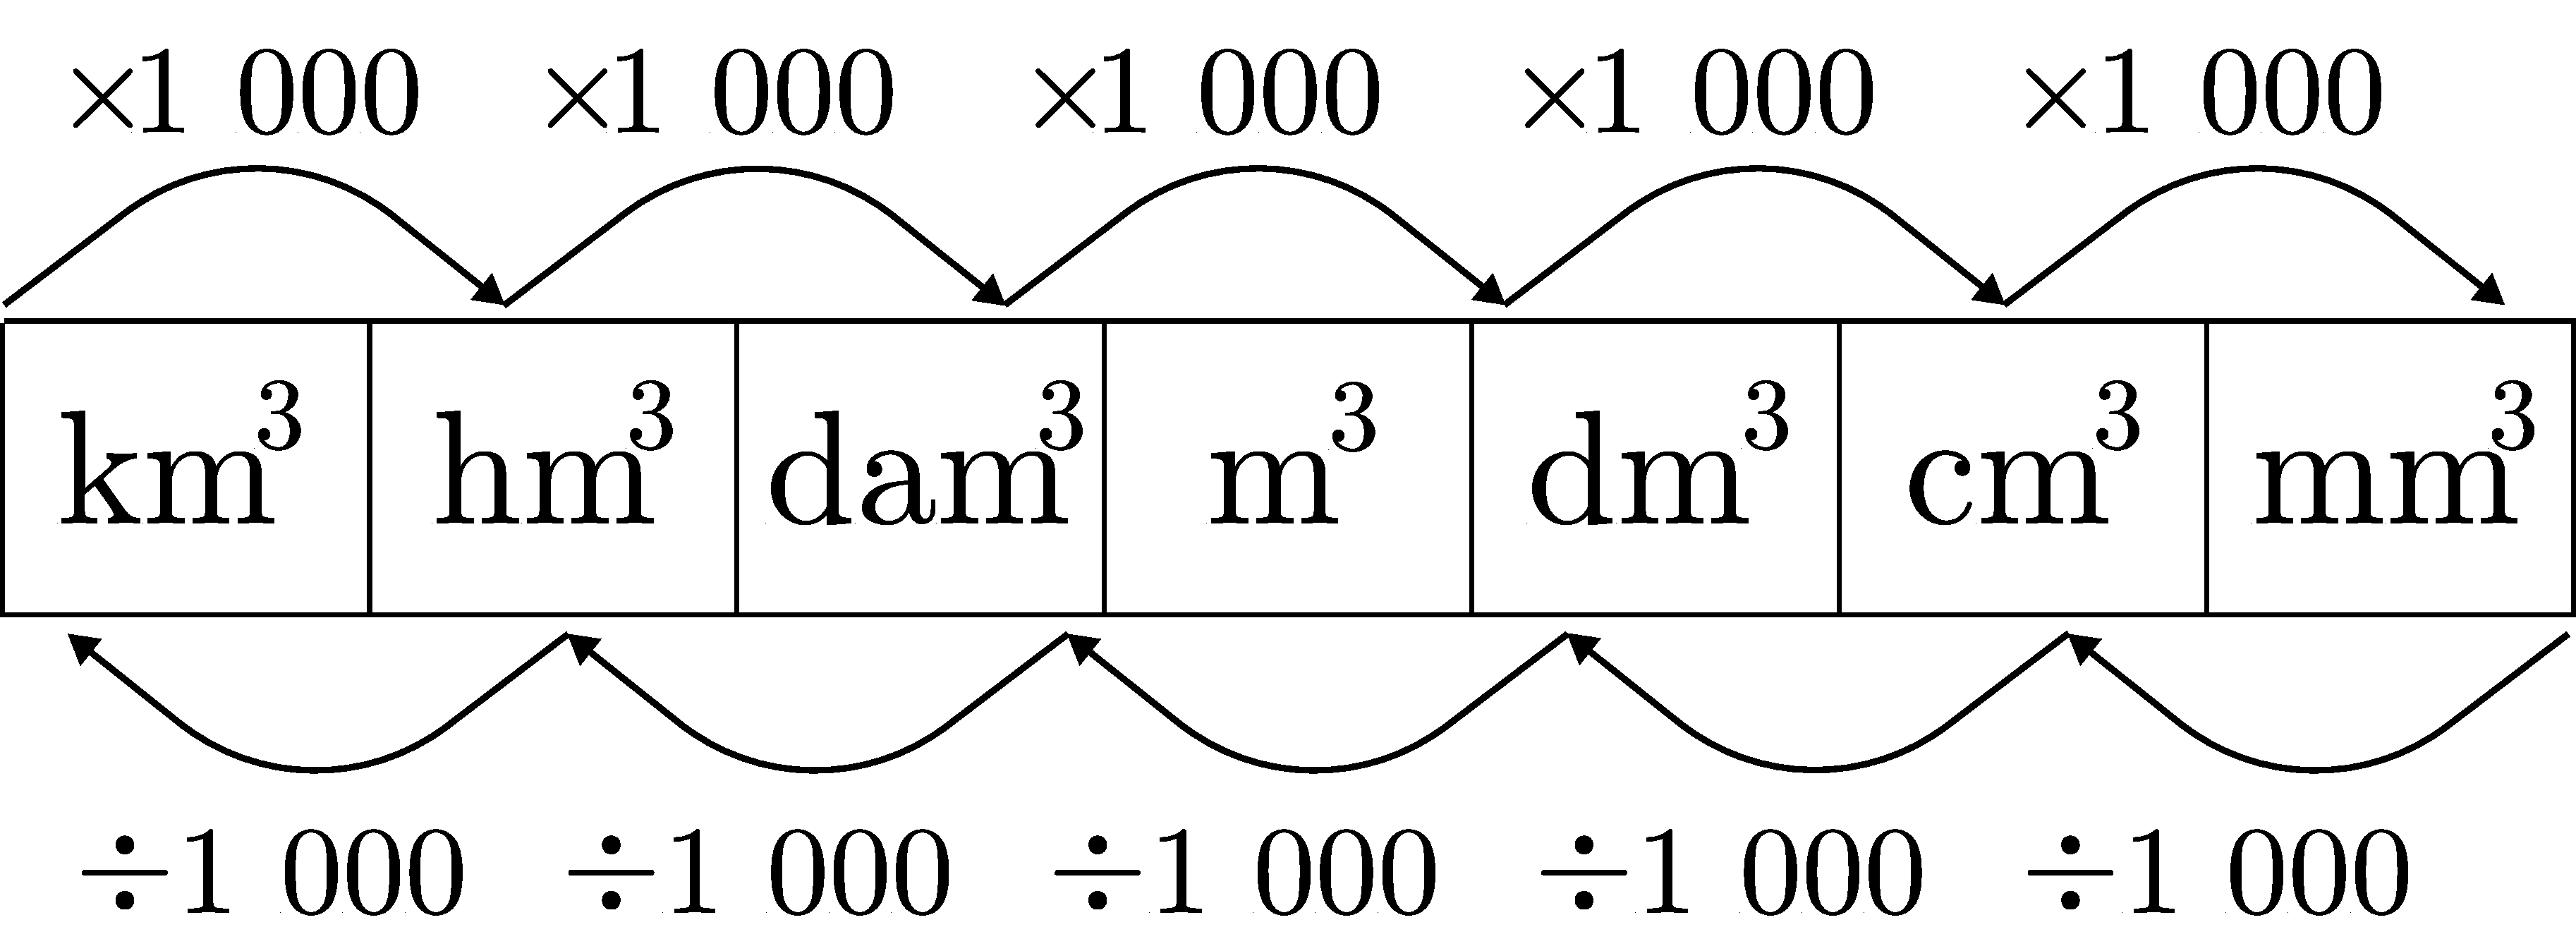
\includegraphics[width=0.4\textwidth]{imagens/matematicaBasica/sistemaDeUnidades/MultiplosDeMetroCubico.pdf}
		\end{figure}
     
\section{Medidas de Capacidade}
As medidas de capacidade são utilizadas para representarem
as grandezas que definem o volume contido em um certo
reservatório. A mais utilizada é o litro ($\mathrm{l}$).
	\\\textbf{Importante:}
	\begin{itemize}
	    \item $1\mathrm{l} = 1\mathrm{dm}^3$
	    \item $1 \mathrm{ml} = 1 \mathrm{cm}^3$
	    \item $10^3 \mathrm{l} = 1 \mathrm{m}^3$
	\end{itemize}
	
\begin{multicols}{2}
	\subsection{Múltiplos de Litro:}
		\begin{itemize}
		    \item Quilolitro ($\mathrm{kl}$) $= 1000 \mathrm{l} = 10^3 \mathrm{l}$
		    \item Hectolitro ($\mathrm{hl}$) $= 100 \mathrm{l} = 10^3 \mathrm{l}$
		    \item Decalitro ($\mathrm{dal}$) $= 10 \mathrm{l} = 10^1\mathrm{l}$
		\end{itemize}

	\subsection{Submúltiplos de Litro:}
		\begin{itemize}
		    \item Decilitro ($\mathrm{dl}$) $= 0,1 \mathrm{l} = 10^{-1}\mathrm{l}$
		    \item Centilitro ($\mathrm{cl}$) $= 0,01 \mathrm{l} = 10^{-2}\mathrm{l}$
		    \item Mililitro ($\mathrm{ml}$) $= 0,001 \mathrm{l} = 10^{-3}\mathrm{l}$
		\end{itemize}
\columnbreak    
     \bigskip
     \noindent   
     \begin{minipage}{\linewidth}
    \centering 
    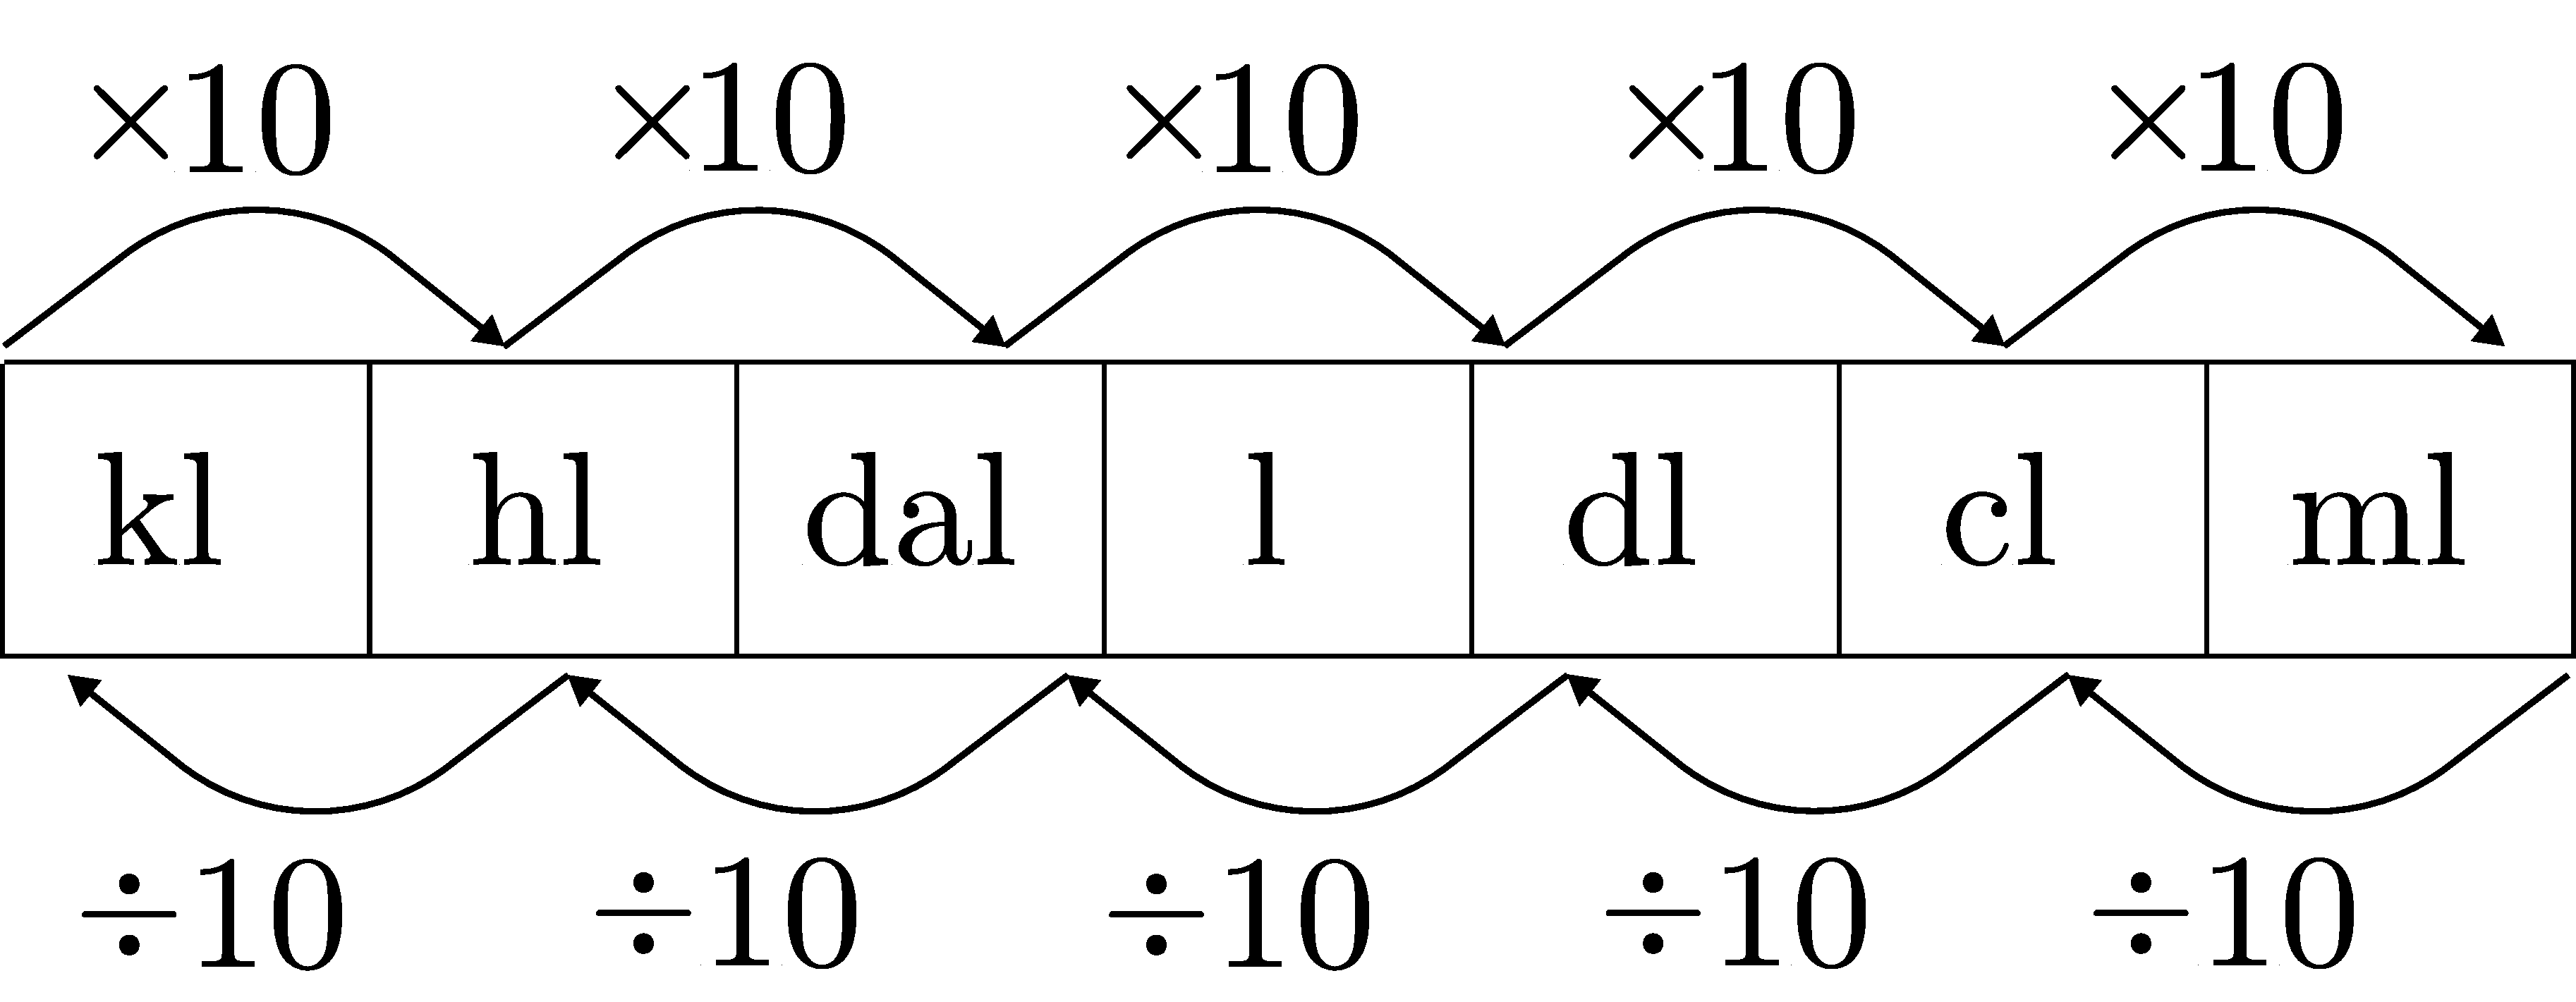
\includegraphics[width=0.8\textwidth]{imagens/matematicaBasica/sistemaDeUnidades/MultiplosDeLitro.pdf}
   %\caption{Múltiplos de litro}
     \end{minipage}
   \end{multicols}  
\section{Medidas de Massa}
As medidas de massa são utilizadas para medir a quantidade
de massa em um corpo. No SI, a unidade fundamental de massa é
o quilograma ($\mathrm{kg}$), embora o grama ($\mathrm{g}$) seja a unidade mais
conveniente para a maioria das medidas de laboratório.
\begin{multicols}{2}
	\subsection{Múltiplos de Grama:}
		\begin{itemize}
		    \item Quilograma ($\mathrm{kg}$) $= 1000 \mathrm{g} = 10^3 \mathrm{g}$
		    \item Hectograma ($\mathrm{hg}$) $= 100 \mathrm{g} = 10^2 \mathrm{g}$
		    \item Decagrama ($\mathrm{dag}$) $= 10 \mathrm{g} = 10^1 \mathrm{g}$
		\end{itemize}
	
	\subsection{Submúltiplos de Grama:}
		\begin{itemize}
		    \item Decigrama ($\mathrm{dg}$) $= 0,1 \mathrm{g} = 10^{-1} \mathrm{g}$
		    \item Centigrama ($\mathrm{cg}$) $= 0,01 \mathrm{g} = 10^{-2} \mathrm{g}$
		    \item Miligrama ($\mathrm{mg}$) $= 0,001 \mathrm{g} = 10^{-3} \mathrm{g}$
		\end{itemize}
		\columnbreak
     \bigskip
     \noindent   % Very important in case that \parindent is not 0pt
     \begin{minipage}{\linewidth}
    \centering 
    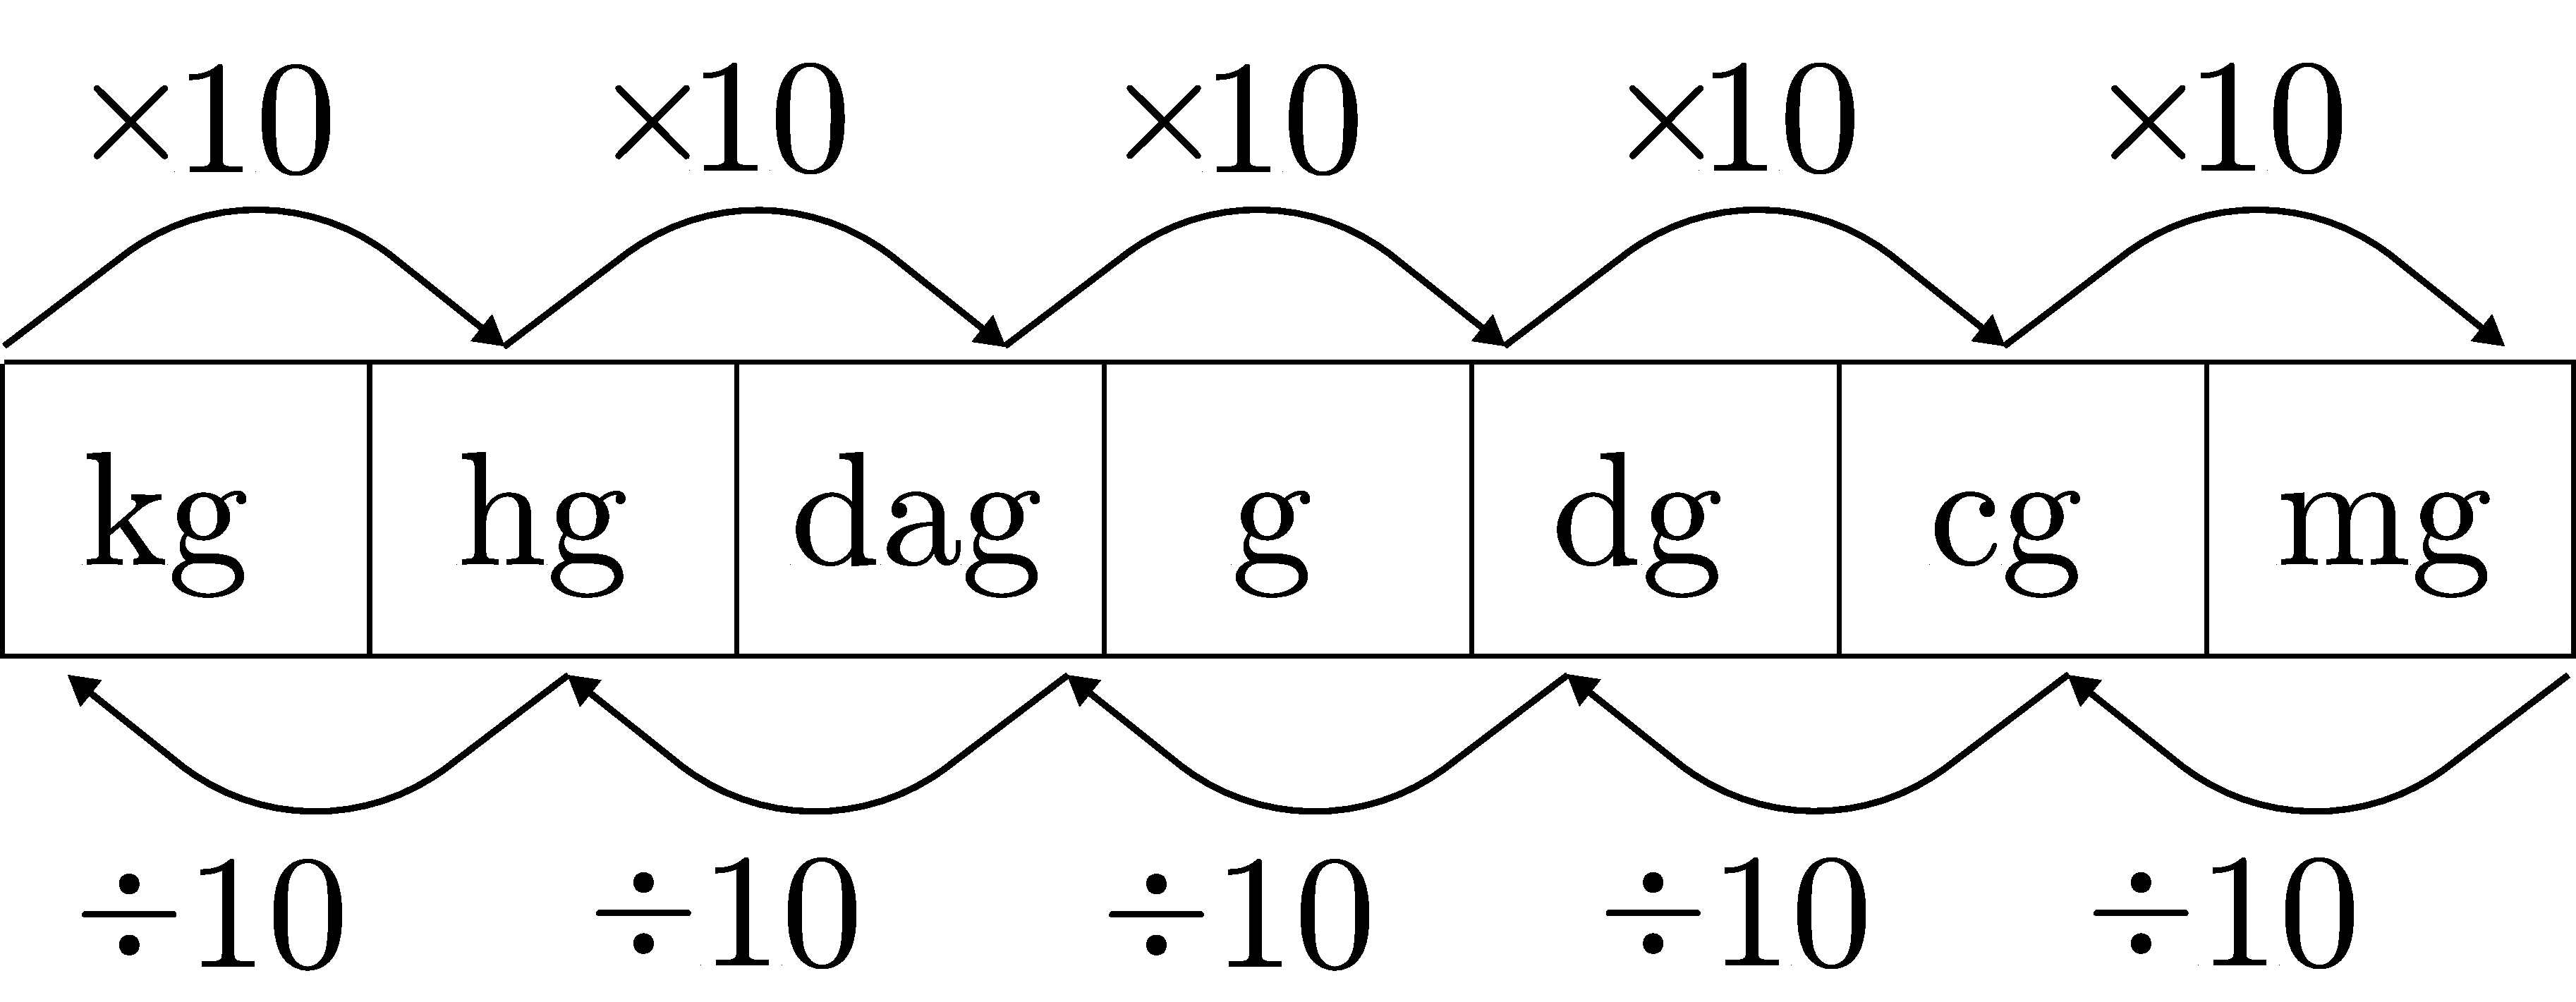
\includegraphics[width=0.8\textwidth]{imagens/matematicaBasica/sistemaDeUnidades/MultiplosDeGrama.pdf}
    %\caption{figure}{Múltiplos de grama}
\end{minipage}
   \end{multicols} 
Existe ainda a unidade especial:
Tonelada ($\mathrm{t}$) $= 1000 \mathrm{kg} = 10^3 \mathrm{kg} = 10^6 \mathrm{g}$

\section{Exercícios}

\begin{exercise}[ENEM 2017]
	Uma empresa especializada em conservação de piscinas utiliza um produto para tratamento da água cujas especificações técnicas sugerem que seja adicionado $1,5 \mathrm{ml}$ desse produto para cada $1000 \mathrm{l}$ de água da piscina. Essa empresa foi contratada para cuidar de uma piscina de base retangular, de profundidade constante igual a $1,7 \mathrm{m}$, com largura e comprimento iguais a $\mathrm{3m}$ e $5 \mathrm{m}$, respectivamente. O nível da lâmina d’água dessa piscina é mantido a $50 \mathrm{cm}$ da borda da piscina.

A quantidade desse produto, em mililitro, que deve ser adicionada a essa piscina de modo a atender às suas especificações técnicas é :
    \begin{description}
        \item[a)] $11,25$
        \item[b)] $27,00$
        \item[c)] $28,80$
        \item[d)] $32,25$
        \item[e)] $49,50$
    \end{description}
\end{exercise}

\begin{exercise}[ENEM 2010]
Um consumidor desconfia que a balança do supermercado não está aferindo corretamente a massa dos produtos. Ao chegar a casa resolve conferir se a balança estava descalibrada. Para isso, utiliza um recipiente provido de escala volumétrica, contendo $1,0$ litro d’água. Ele coloca uma porção dos legumes que comprou dentro do recipiente e observa que a água atinge a marca de $1,5$ litro e também que a porção não ficara totalmente submersa, com $1/3$ de seu volume fora d’água. Para concluir o teste, o consumidor, com ajuda da internet, verifica que a  densidade dos legumes, em questão, é a metade da densidade da água, onde, $ \rho \cdot \textrm{água} = 1 \mathrm{g/cm^{3}}$.

No supermercado a balança registrou a massa da porção de legumes igual a $0,500 \mathrm{kg}$ (meio quilograma).Considerando que o método adotado tenha boa precisão, o consumidor concluiu que a balança estava descalibrada e deveria ter registrado a massa da porção de legumes igual a:

    \begin{description}
        \item[a)] $0,073 \mathrm{ kg}$
        \item[b)] $0,167 \mathrm{ kg}$
        \item[c)] $0,250 \mathrm{ kg}$
        \item[d)] $0,375 \mathrm{ kg}$
        \item[e)] $0,750 \mathrm{ kg}$
    \end{description}
\end{exercise}

\begin{exercise}[ENEM 2011]
Um mecânico de uma equipe de corrida necessita que as seguintes medidas realizadas em um carro sejam obtidas em metros:

\begin{description}
    \item[a] distância a entre os eixos dianteiro e traseiro;
    \item[b] altura b entre o solo e o encosto do piloto. 
\end{description}
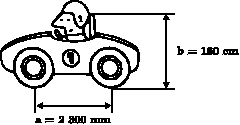
\includegraphics[width=0.4\textwidth]{imagens/matematicaBasica/sistemaDeUnidades/carro.pdf}\\
Ao optar pelas medidas $\mathrm{a}$ e $\mathrm{b}$ em metros, obtêm-se, respectivamente,

    \begin{description}
        \item[a)] $0,23 \textrm{ e } 0,16$
        \item[b)] $2,3 \textrm{ e } 1,6$
        \item[c)] $23 \textrm{ e } 16$
        \item[d)] $230 \textrm{ e } 160$
        \item[e)] $2300 \textrm{ e } 1600$
    \end{description}

\end{exercise}

\begin{exercise}[ENEM 2011]
Um aluno de Ensino Médio vai até o açougue, a pedido de seus pais, comprar $5 \mathrm{kg}$ de carne para um churrasco em sua casa. Além da carne, ele compra $8$ litros de refrigerante para oferecer aos convidados. Qual das alternativas a seguir possui os valores da quantidade de carne e de refrigerante, respectivamente, nas unidades tonelada ($\mathrm{t}$) e mililitro ($\mathrm{ml}$)?

    \begin{description}
        \item[a)] $0,005 \mathrm{t} \textrm{ e } 0,008 \mathrm{ml}$
        \item[b)] $5000 \mathrm{t} \textrm{ e } 0,008 \mathrm{ml}$
        \item[c)] $0,005 \mathrm{t} \textrm{ e } 8000 \mathrm{ml}$
        \item[d)] $5000 \mathrm{t} \textrm{ e } 8000 \mathrm{ml}$
        \item[e)] $0,005 \mathrm{t} \textrm{ e } 0,8 \mathrm{ml}$
    \end{description}

\end{exercise}
